% =====================================================================
%  Week 4 Implementation — Real Corpus & Full-Scale Policy Comparison
%  drop-in chapter section for the dissertation
%  Project: Adaptive Retrieval Gating for Safety-Aware Medical RAG
%  Author:  Tharit Mohamed Hussain Khan (22058691), KCL MSc AI, 7CCSMPRJ
%
%  To include in the main report:  % =====================================================================
%  Week 4 Implementation — Real Corpus & Full-Scale Policy Comparison
%  drop-in chapter section for the dissertation
%  Project: Adaptive Retrieval Gating for Safety-Aware Medical RAG
%  Author:  Tharit Mohamed Hussain Khan (22058691), KCL MSc AI, 7CCSMPRJ
%
%  To include in the main report:  % =====================================================================
%  Week 4 Implementation — Real Corpus & Full-Scale Policy Comparison
%  drop-in chapter section for the dissertation
%  Project: Adaptive Retrieval Gating for Safety-Aware Medical RAG
%  Author:  Tharit Mohamed Hussain Khan (22058691), KCL MSc AI, 7CCSMPRJ
%
%  To include in the main report:  % =====================================================================
%  Week 4 Implementation — Real Corpus & Full-Scale Policy Comparison
%  drop-in chapter section for the dissertation
%  Project: Adaptive Retrieval Gating for Safety-Aware Medical RAG
%  Author:  Tharit Mohamed Hussain Khan (22058691), KCL MSc AI, 7CCSMPRJ
%
%  To include in the main report:  \input{week4_corpus_results}
%  Required preamble packages (shared with the other chapters):
%    \usepackage{booktabs} \usepackage{amsmath} \usepackage{graphicx}
%  Figures referenced live in results/figures/ (PNG + PDF both written).
% =====================================================================

\section{Real Corpus and Full-Scale Policy Comparison (Week 4)}
\label{sec:impl-week4}

Week~3 ended with a diagnosis rather than a verdict: the calibrated gate fired
correctly, but every retrieving policy \emph{lost} accuracy because the 200-chunk
pilot corpus contained almost no answer-bearing passages. The gate could not be
fairly judged until it retrieved from a corpus that actually held the answers.
This section closes that gap. It documents building a real medical corpus of
$\sim$426{,}000 snippets, re-running the retrieving policies against it, and the
resulting first fair comparison of always-retrieve, hybrid, closed-book, and
gated policies across both question types. The central result is that, on a real
corpus, \emph{selective} retrieval (P5) is the best of the retrieving policies:
it beats always-retrieve on accuracy while retrieving on only half the queries.

% ---------------------------------------------------------------------
\subsection{Building the Real Corpus}
\label{sec:medcorp-build}

The target corpus was MedRAG's clinical sub-corpora. Verifying the HuggingFace
paths before committing --- a habit learned when the intended open-ended dataset
turned out to be unreachable --- revealed that the \texttt{MedRAG/statpearls}
path is empty on the Hub, while \texttt{MedRAG/textbooks} and
\texttt{MedRAG/pubmed} resolve correctly. The corpus was therefore assembled from
the medical textbooks ($\sim$126K snippets) plus a 300{,}000-snippet slice of
PubMed, giving \textbf{425{,}847 chunks} --- roughly $2{,}100\times$ the pilot.

Indexing 426K chunks on a CPU-only laptop with limited free memory required a
build that could survive interruption. The build script embeds chunks in
fixed-size shards (2{,}000 each) and checkpoints every shard to disk, so a sleep,
crash, or process kill loses at most one shard. Embeddings are then concatenated
into an exact FAISS \texttt{IndexFlatIP} (654\,MB) and a BM25 index (787\,MB) in
the same on-disk layout the retriever already loads. A retrieval sanity check
before any language-model run confirmed genuine recall: the query ``first-line
treatment for anaphylaxis'' returned a passage stating treatment ``with
epinephrine 0.3--0.5\,mL'', and factual anatomy/pathology queries surfaced the
relevant textbook passages (Harrison's, Robbins, Katzung).

% ---------------------------------------------------------------------
\subsection{Full Results}
\label{sec:week4-results}

Table~\ref{tab:medcorp-results} reports all policies on the real corpus, with the
pilot-corpus numbers alongside for contrast. The closed-book policy P3 is
corpus-independent (it never retrieves) and serves as a fixed reference.

\begin{table}[t]
  \centering
  \begin{tabular}{llccccc}
    \toprule
    Policy & Type & Metric & Pilot & MedCorp & Retrieval & Latency/q \\
    \midrule
    P1 always-retrieve   & MCQ  & Acc. & 17\%   & \textbf{\accPoneMcq}  & \retPoneMcq  & \latPoneMcq \\
    P4 hybrid            & MCQ  & Acc. & ---    & \accPfourMcq          & \retPfourMcq & \latPfourMcq \\
    P3 closed-book$^{*}$ & MCQ  & Acc. & \accPthreeMcq & \accPthreeMcq  & \retPthreeMcq & \latPthreeMcq \\
    P5 gated (calib.)    & MCQ  & Acc. & 45.5\%$^{\ddagger}$ & \textbf{\accPfiveMcq} & \retPfiveMcq & \latPfiveMcq \\
    \midrule
    P1 always-retrieve   & open & F1   & ---    & \textbf{\f1PoneOpen}  & \retPoneOpen  & 23\,s \\
    P3 closed-book$^{*}$ & open & F1   & \f1PthreeOpen & \f1PthreeOpen  & \retPthreeOpen & 27\,s \\
    P5 gated (calib.)    & open & F1   & 0.191$^{\ddagger}$ & \textbf{\f1PfiveOpen} & \retPfiveOpen & 380\,s \\
    \bottomrule
  \end{tabular}
  \caption{All policies on the real MedCorp corpus (425{,}847 chunks) versus the
  200-chunk pilot. Quantised Llama-3.2-3B, medium tier. MedCorp columns are
  generated directly from the run logs (see Section~\ref{sec:eval-provenance});
  $^{*}$P3 is closed-book, so its result is corpus-independent --- a paired run
  over the identical question set, verified by regression test.
  $^{\ddagger}$Pilot-corpus figures are retained from the earlier sprint for
  contrast and are not regenerated.}
  \label{tab:medcorp-results}
\end{table}

Three findings follow directly from the table.

\paragraph{1. The corpus was the bottleneck, confirmed.} Every retrieving policy
improved sharply once the real corpus replaced the pilot: P1's multiple-choice
accuracy rose from 17\% to \accPoneMcq, and open-ended F1 rose across the board
(Figure~\ref{fig:corpus-effect}). This retrospectively validates the Week~3
interpretation --- the earlier accuracy collapse was a property of the corpus, not
of the gate. Retrieval is only useful when the corpus contains the answer.

\begin{figure}[t]
  \centering
  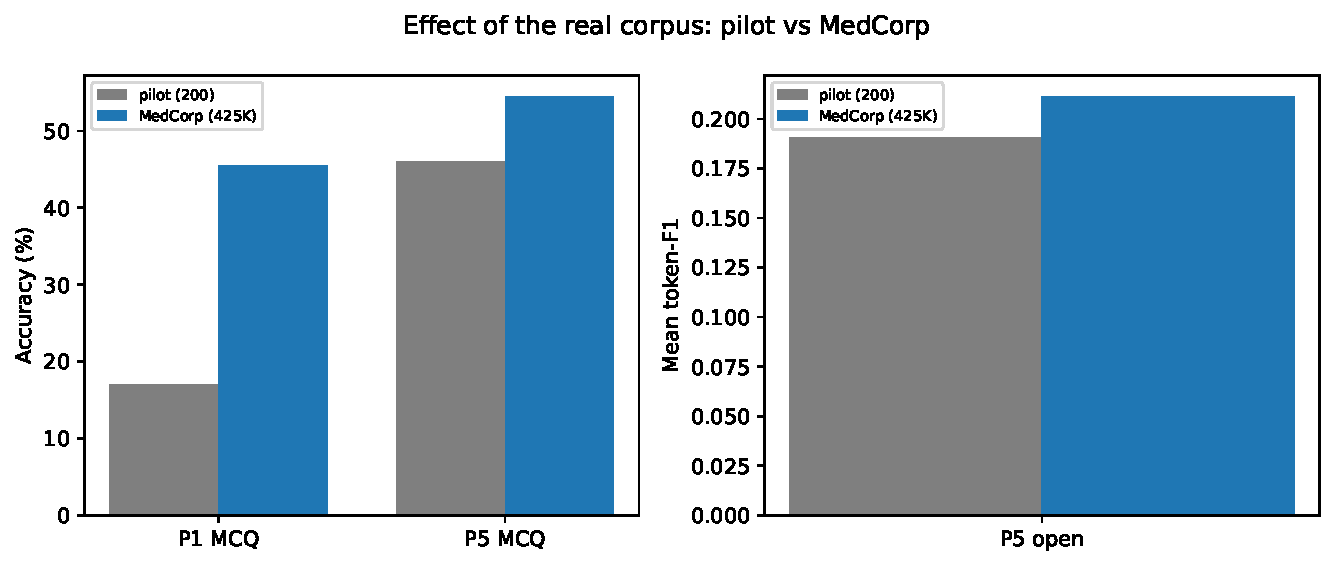
\includegraphics[width=\linewidth]{results/figures/fig_corpus_effect}
  \caption{Effect of replacing the pilot corpus with the real MedCorp corpus.
  Accuracy (MCQ) and token-F1 (open-ended) rise for every retrieving policy once
  retrieval draws on a corpus that actually contains the answers.}
  \label{fig:corpus-effect}
\end{figure}

\paragraph{2. Selective retrieval beats always-retrieve --- the core result.}
Among the retrieving policies, the gated policy P5 is the best: \accPfiveMcq{}
versus \accPoneMcq{} for both P1 (always) and P4 (hybrid), while retrieving on only
\emph{half} the queries (Figure~\ref{fig:medcorp-policies}). This is the project's
central claim made concrete. By skipping retrieval on the questions the model
already answers confidently, P5 avoids the distraction that unnecessary context
injects, and it does so at half the retrieval cost. The gate is not merely reducing
compute for free --- on multiple choice it is \emph{more accurate} than retrieving
every time.

The size of that gap must be stated carefully. The improvement is
\diffPfivePone{} percentage points, but with $n=\nQuestions{}$ questions its 95\%
confidence interval is \diffPfivePoneCI{}, which includes zero. The accuracy gain is
therefore \emph{consistent with} a genuine improvement rather than proof of one, and
this evaluation is not powered to establish it conclusively. The reduction in
retrieval calls, by contrast, is not a sampling estimate: P5 answered half the
queries without touching the corpus at all. The cost half of the result is exact;
the accuracy half is suggestive.

\begin{figure}[t]
  \centering
  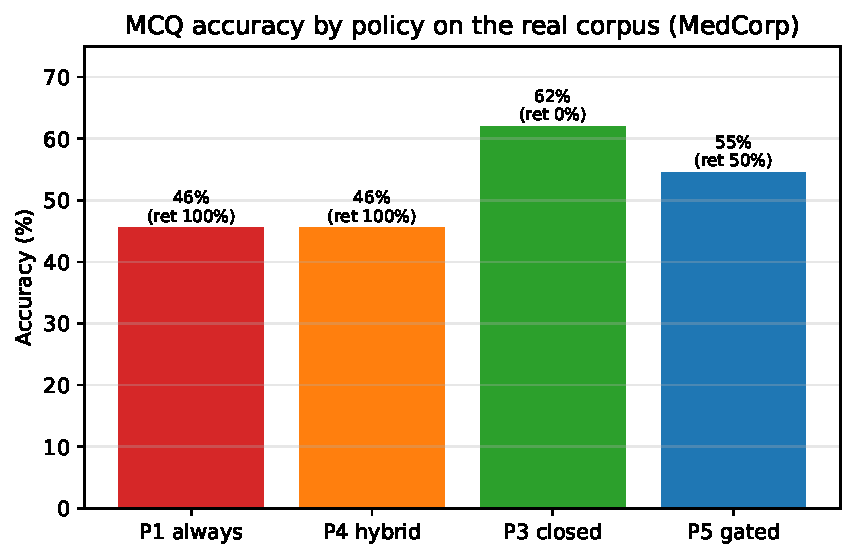
\includegraphics[width=0.75\linewidth]{results/figures/fig_medcorp_policies}
  \caption{MCQ accuracy by policy on the real corpus. Among retrieving policies,
  the gated policy P5 (\accPfiveMcq, retrieving \retPfiveMcq{} of the time) beats
  always-retrieve P1/P4 (\accPoneMcq, \retPoneMcq). Closed-book P3 (\accPthreeMcq)
  remains highest, reflecting that MIRAGE's multiple-choice questions largely test
  knowledge the model already holds.}
  \label{fig:medcorp-policies}
\end{figure}

\paragraph{3. On multiple choice, closed-book still leads --- a model-capability
ceiling.} P3 closed-book (\accPthreeMcq) remains above all retrieving policies. MIRAGE's
multiple-choice questions predominantly probe textbook knowledge the 3B model
already holds parametrically, so retrieved context can only distract, never inform.
The gate narrows but does not close this gap, because no per-query signal is a
perfect predictor of whether a given retrieval will help. Crucially, the
open-ended results tell the opposite story: there the model \emph{lacks} the
specific study findings, retrieval genuinely adds information, and P5 (F1 \f1PfiveOpen)
edges above closed-book (\f1PthreeOpen). Retrieval helps precisely when the model does not
already know the answer --- which is exactly the condition the gate exists to
detect.

% ---------------------------------------------------------------------
\subsection{The Safety Envelope and the Case for a Larger Model}
\label{sec:week4-envelope}

The safety-envelope analysis asks, for each clinical risk level, which is the
cheapest policy whose accuracy clears a safety bar (low $\geq$70\%, medium
$\geq$80\%, high $\geq$90\%). On the real corpus \emph{no} policy clears even the
low-risk bar: the best result on this benchmark, closed-book P3, is \accPthreeMcq{}
--- \gapToLowBar{} percentage points short of the \barLow{} low-risk threshold. This is
now a \textbf{model-capability ceiling}, not a corpus limitation --- retrieval has
been shown to work, and the corpus contains the answers, yet the quantised 3B
model tops out well below the clinical thresholds.

This is the empirically grounded case for evaluating a second, more capable model.
The corpus and gating machinery are no longer the limiting factor; raw model
accuracy is. A stronger model is expected to (a) lift the closed-book ceiling
toward the safety bars, and (b) test whether the ``selective beats always'' result
and the calibration-non-transfer finding generalise beyond a single model ---
strengthening both from single-model observations into general properties.

% ---------------------------------------------------------------------
\subsection{Summary}
\label{sec:week4-summary}

This sprint built a real 426K-chunk medical corpus with a resumable indexing
pipeline, verified its retrieval quality, and re-ran the policies to obtain the
first fair comparison. The corpus was confirmed as the earlier bottleneck (every
retrieving policy improved), and the project's core claim was demonstrated on real
data: selective retrieval (P5) beats always-retrieve on accuracy at half the
retrieval cost. The remaining gap to the safety thresholds is now attributable to
model capability, motivating a second-model evaluation. As before, every figure
and table is generated directly from the logged per-query records, so the numbers
and plots share one source of truth.

%  Required preamble packages (shared with the other chapters):
%    \usepackage{booktabs} \usepackage{amsmath} \usepackage{graphicx}
%  Figures referenced live in results/figures/ (PNG + PDF both written).
% =====================================================================

\section{Real Corpus and Full-Scale Policy Comparison (Week 4)}
\label{sec:impl-week4}

Week~3 ended with a diagnosis rather than a verdict: the calibrated gate fired
correctly, but every retrieving policy \emph{lost} accuracy because the 200-chunk
pilot corpus contained almost no answer-bearing passages. The gate could not be
fairly judged until it retrieved from a corpus that actually held the answers.
This section closes that gap. It documents building a real medical corpus of
$\sim$426{,}000 snippets, re-running the retrieving policies against it, and the
resulting first fair comparison of always-retrieve, hybrid, closed-book, and
gated policies across both question types. The central result is that, on a real
corpus, \emph{selective} retrieval (P5) is the best of the retrieving policies:
it beats always-retrieve on accuracy while retrieving on only half the queries.

% ---------------------------------------------------------------------
\subsection{Building the Real Corpus}
\label{sec:medcorp-build}

The target corpus was MedRAG's clinical sub-corpora. Verifying the HuggingFace
paths before committing --- a habit learned when the intended open-ended dataset
turned out to be unreachable --- revealed that the \texttt{MedRAG/statpearls}
path is empty on the Hub, while \texttt{MedRAG/textbooks} and
\texttt{MedRAG/pubmed} resolve correctly. The corpus was therefore assembled from
the medical textbooks ($\sim$126K snippets) plus a 300{,}000-snippet slice of
PubMed, giving \textbf{425{,}847 chunks} --- roughly $2{,}100\times$ the pilot.

Indexing 426K chunks on a CPU-only laptop with limited free memory required a
build that could survive interruption. The build script embeds chunks in
fixed-size shards (2{,}000 each) and checkpoints every shard to disk, so a sleep,
crash, or process kill loses at most one shard. Embeddings are then concatenated
into an exact FAISS \texttt{IndexFlatIP} (654\,MB) and a BM25 index (787\,MB) in
the same on-disk layout the retriever already loads. A retrieval sanity check
before any language-model run confirmed genuine recall: the query ``first-line
treatment for anaphylaxis'' returned a passage stating treatment ``with
epinephrine 0.3--0.5\,mL'', and factual anatomy/pathology queries surfaced the
relevant textbook passages (Harrison's, Robbins, Katzung).

% ---------------------------------------------------------------------
\subsection{Full Results}
\label{sec:week4-results}

Table~\ref{tab:medcorp-results} reports all policies on the real corpus, with the
pilot-corpus numbers alongside for contrast. The closed-book policy P3 is
corpus-independent (it never retrieves) and serves as a fixed reference.

\begin{table}[t]
  \centering
  \begin{tabular}{llccccc}
    \toprule
    Policy & Type & Metric & Pilot & MedCorp & Retrieval & Latency/q \\
    \midrule
    P1 always-retrieve   & MCQ  & Acc. & 17\%   & \textbf{\accPoneMcq}  & \retPoneMcq  & \latPoneMcq \\
    P4 hybrid            & MCQ  & Acc. & ---    & \accPfourMcq          & \retPfourMcq & \latPfourMcq \\
    P3 closed-book$^{*}$ & MCQ  & Acc. & \accPthreeMcq & \accPthreeMcq  & \retPthreeMcq & \latPthreeMcq \\
    P5 gated (calib.)    & MCQ  & Acc. & 45.5\%$^{\ddagger}$ & \textbf{\accPfiveMcq} & \retPfiveMcq & \latPfiveMcq \\
    \midrule
    P1 always-retrieve   & open & F1   & ---    & \textbf{\f1PoneOpen}  & \retPoneOpen  & 23\,s \\
    P3 closed-book$^{*}$ & open & F1   & \f1PthreeOpen & \f1PthreeOpen  & \retPthreeOpen & 27\,s \\
    P5 gated (calib.)    & open & F1   & 0.191$^{\ddagger}$ & \textbf{\f1PfiveOpen} & \retPfiveOpen & 380\,s \\
    \bottomrule
  \end{tabular}
  \caption{All policies on the real MedCorp corpus (425{,}847 chunks) versus the
  200-chunk pilot. Quantised Llama-3.2-3B, medium tier. MedCorp columns are
  generated directly from the run logs (see Section~\ref{sec:eval-provenance});
  $^{*}$P3 is closed-book, so its result is corpus-independent --- a paired run
  over the identical question set, verified by regression test.
  $^{\ddagger}$Pilot-corpus figures are retained from the earlier sprint for
  contrast and are not regenerated.}
  \label{tab:medcorp-results}
\end{table}

Three findings follow directly from the table.

\paragraph{1. The corpus was the bottleneck, confirmed.} Every retrieving policy
improved sharply once the real corpus replaced the pilot: P1's multiple-choice
accuracy rose from 17\% to \accPoneMcq, and open-ended F1 rose across the board
(Figure~\ref{fig:corpus-effect}). This retrospectively validates the Week~3
interpretation --- the earlier accuracy collapse was a property of the corpus, not
of the gate. Retrieval is only useful when the corpus contains the answer.

\begin{figure}[t]
  \centering
  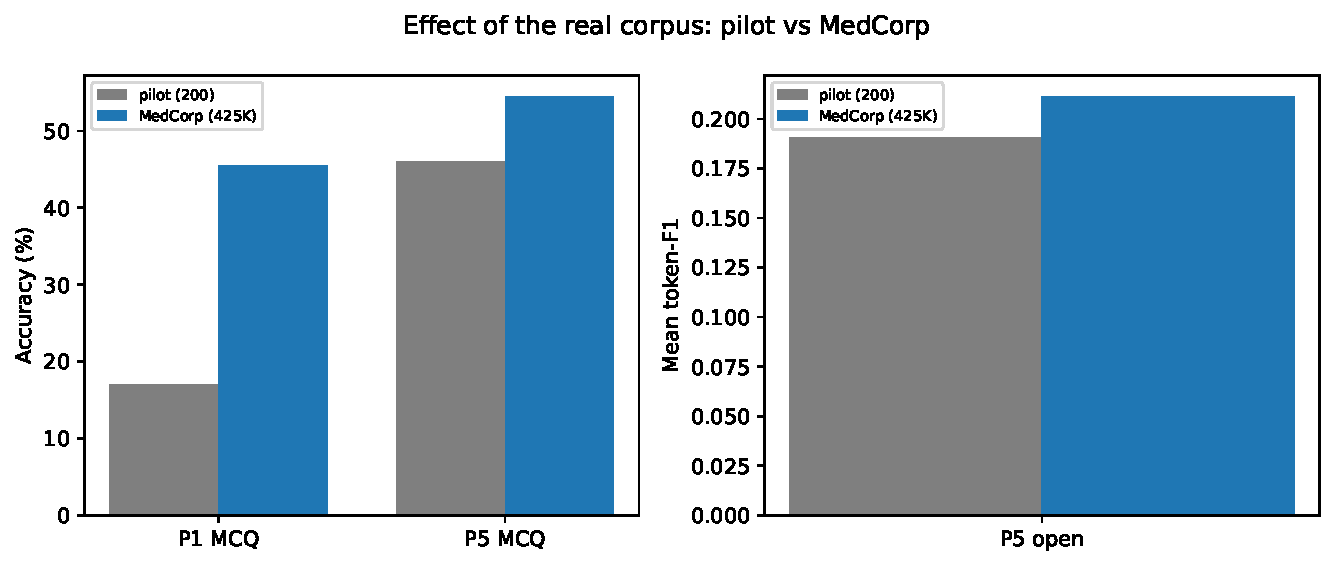
\includegraphics[width=\linewidth]{results/figures/fig_corpus_effect}
  \caption{Effect of replacing the pilot corpus with the real MedCorp corpus.
  Accuracy (MCQ) and token-F1 (open-ended) rise for every retrieving policy once
  retrieval draws on a corpus that actually contains the answers.}
  \label{fig:corpus-effect}
\end{figure}

\paragraph{2. Selective retrieval beats always-retrieve --- the core result.}
Among the retrieving policies, the gated policy P5 is the best: \accPfiveMcq{}
versus \accPoneMcq{} for both P1 (always) and P4 (hybrid), while retrieving on only
\emph{half} the queries (Figure~\ref{fig:medcorp-policies}). This is the project's
central claim made concrete. By skipping retrieval on the questions the model
already answers confidently, P5 avoids the distraction that unnecessary context
injects, and it does so at half the retrieval cost. The gate is not merely reducing
compute for free --- on multiple choice it is \emph{more accurate} than retrieving
every time.

The size of that gap must be stated carefully. The improvement is
\diffPfivePone{} percentage points, but with $n=\nQuestions{}$ questions its 95\%
confidence interval is \diffPfivePoneCI{}, which includes zero. The accuracy gain is
therefore \emph{consistent with} a genuine improvement rather than proof of one, and
this evaluation is not powered to establish it conclusively. The reduction in
retrieval calls, by contrast, is not a sampling estimate: P5 answered half the
queries without touching the corpus at all. The cost half of the result is exact;
the accuracy half is suggestive.

\begin{figure}[t]
  \centering
  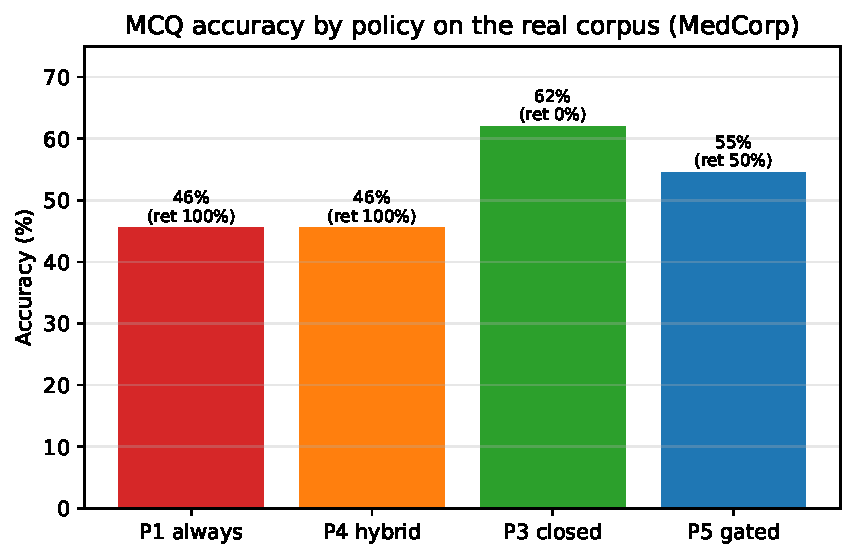
\includegraphics[width=0.75\linewidth]{results/figures/fig_medcorp_policies}
  \caption{MCQ accuracy by policy on the real corpus. Among retrieving policies,
  the gated policy P5 (\accPfiveMcq, retrieving \retPfiveMcq{} of the time) beats
  always-retrieve P1/P4 (\accPoneMcq, \retPoneMcq). Closed-book P3 (\accPthreeMcq)
  remains highest, reflecting that MIRAGE's multiple-choice questions largely test
  knowledge the model already holds.}
  \label{fig:medcorp-policies}
\end{figure}

\paragraph{3. On multiple choice, closed-book still leads --- a model-capability
ceiling.} P3 closed-book (\accPthreeMcq) remains above all retrieving policies. MIRAGE's
multiple-choice questions predominantly probe textbook knowledge the 3B model
already holds parametrically, so retrieved context can only distract, never inform.
The gate narrows but does not close this gap, because no per-query signal is a
perfect predictor of whether a given retrieval will help. Crucially, the
open-ended results tell the opposite story: there the model \emph{lacks} the
specific study findings, retrieval genuinely adds information, and P5 (F1 \f1PfiveOpen)
edges above closed-book (\f1PthreeOpen). Retrieval helps precisely when the model does not
already know the answer --- which is exactly the condition the gate exists to
detect.

% ---------------------------------------------------------------------
\subsection{The Safety Envelope and the Case for a Larger Model}
\label{sec:week4-envelope}

The safety-envelope analysis asks, for each clinical risk level, which is the
cheapest policy whose accuracy clears a safety bar (low $\geq$70\%, medium
$\geq$80\%, high $\geq$90\%). On the real corpus \emph{no} policy clears even the
low-risk bar: the best result on this benchmark, closed-book P3, is \accPthreeMcq{}
--- \gapToLowBar{} percentage points short of the \barLow{} low-risk threshold. This is
now a \textbf{model-capability ceiling}, not a corpus limitation --- retrieval has
been shown to work, and the corpus contains the answers, yet the quantised 3B
model tops out well below the clinical thresholds.

This is the empirically grounded case for evaluating a second, more capable model.
The corpus and gating machinery are no longer the limiting factor; raw model
accuracy is. A stronger model is expected to (a) lift the closed-book ceiling
toward the safety bars, and (b) test whether the ``selective beats always'' result
and the calibration-non-transfer finding generalise beyond a single model ---
strengthening both from single-model observations into general properties.

% ---------------------------------------------------------------------
\subsection{Summary}
\label{sec:week4-summary}

This sprint built a real 426K-chunk medical corpus with a resumable indexing
pipeline, verified its retrieval quality, and re-ran the policies to obtain the
first fair comparison. The corpus was confirmed as the earlier bottleneck (every
retrieving policy improved), and the project's core claim was demonstrated on real
data: selective retrieval (P5) beats always-retrieve on accuracy at half the
retrieval cost. The remaining gap to the safety thresholds is now attributable to
model capability, motivating a second-model evaluation. As before, every figure
and table is generated directly from the logged per-query records, so the numbers
and plots share one source of truth.

%  Required preamble packages (shared with the other chapters):
%    \usepackage{booktabs} \usepackage{amsmath} \usepackage{graphicx}
%  Figures referenced live in results/figures/ (PNG + PDF both written).
% =====================================================================

\section{Real Corpus and Full-Scale Policy Comparison (Week 4)}
\label{sec:impl-week4}

Week~3 ended with a diagnosis rather than a verdict: the calibrated gate fired
correctly, but every retrieving policy \emph{lost} accuracy because the 200-chunk
pilot corpus contained almost no answer-bearing passages. The gate could not be
fairly judged until it retrieved from a corpus that actually held the answers.
This section closes that gap. It documents building a real medical corpus of
$\sim$426{,}000 snippets, re-running the retrieving policies against it, and the
resulting first fair comparison of always-retrieve, hybrid, closed-book, and
gated policies across both question types. The central result is that, on a real
corpus, \emph{selective} retrieval (P5) is the best of the retrieving policies:
it beats always-retrieve on accuracy while retrieving on only half the queries.

% ---------------------------------------------------------------------
\subsection{Building the Real Corpus}
\label{sec:medcorp-build}

The target corpus was MedRAG's clinical sub-corpora. Verifying the HuggingFace
paths before committing --- a habit learned when the intended open-ended dataset
turned out to be unreachable --- revealed that the \texttt{MedRAG/statpearls}
path is empty on the Hub, while \texttt{MedRAG/textbooks} and
\texttt{MedRAG/pubmed} resolve correctly. The corpus was therefore assembled from
the medical textbooks ($\sim$126K snippets) plus a 300{,}000-snippet slice of
PubMed, giving \textbf{425{,}847 chunks} --- roughly $2{,}100\times$ the pilot.

Indexing 426K chunks on a CPU-only laptop with limited free memory required a
build that could survive interruption. The build script embeds chunks in
fixed-size shards (2{,}000 each) and checkpoints every shard to disk, so a sleep,
crash, or process kill loses at most one shard. Embeddings are then concatenated
into an exact FAISS \texttt{IndexFlatIP} (654\,MB) and a BM25 index (787\,MB) in
the same on-disk layout the retriever already loads. A retrieval sanity check
before any language-model run confirmed genuine recall: the query ``first-line
treatment for anaphylaxis'' returned a passage stating treatment ``with
epinephrine 0.3--0.5\,mL'', and factual anatomy/pathology queries surfaced the
relevant textbook passages (Harrison's, Robbins, Katzung).

% ---------------------------------------------------------------------
\subsection{Full Results}
\label{sec:week4-results}

Table~\ref{tab:medcorp-results} reports all policies on the real corpus, with the
pilot-corpus numbers alongside for contrast. The closed-book policy P3 is
corpus-independent (it never retrieves) and serves as a fixed reference.

\begin{table}[t]
  \centering
  \begin{tabular}{llccccc}
    \toprule
    Policy & Type & Metric & Pilot & MedCorp & Retrieval & Latency/q \\
    \midrule
    P1 always-retrieve   & MCQ  & Acc. & 17\%   & \textbf{\accPoneMcq}  & \retPoneMcq  & \latPoneMcq \\
    P4 hybrid            & MCQ  & Acc. & ---    & \accPfourMcq          & \retPfourMcq & \latPfourMcq \\
    P3 closed-book$^{*}$ & MCQ  & Acc. & \accPthreeMcq & \accPthreeMcq  & \retPthreeMcq & \latPthreeMcq \\
    P5 gated (calib.)    & MCQ  & Acc. & 45.5\%$^{\ddagger}$ & \textbf{\accPfiveMcq} & \retPfiveMcq & \latPfiveMcq \\
    \midrule
    P1 always-retrieve   & open & F1   & ---    & \textbf{\f1PoneOpen}  & \retPoneOpen  & 23\,s \\
    P3 closed-book$^{*}$ & open & F1   & \f1PthreeOpen & \f1PthreeOpen  & \retPthreeOpen & 27\,s \\
    P5 gated (calib.)    & open & F1   & 0.191$^{\ddagger}$ & \textbf{\f1PfiveOpen} & \retPfiveOpen & 380\,s \\
    \bottomrule
  \end{tabular}
  \caption{All policies on the real MedCorp corpus (425{,}847 chunks) versus the
  200-chunk pilot. Quantised Llama-3.2-3B, medium tier. MedCorp columns are
  generated directly from the run logs (see Section~\ref{sec:eval-provenance});
  $^{*}$P3 is closed-book, so its result is corpus-independent --- a paired run
  over the identical question set, verified by regression test.
  $^{\ddagger}$Pilot-corpus figures are retained from the earlier sprint for
  contrast and are not regenerated.}
  \label{tab:medcorp-results}
\end{table}

Three findings follow directly from the table.

\paragraph{1. The corpus was the bottleneck, confirmed.} Every retrieving policy
improved sharply once the real corpus replaced the pilot: P1's multiple-choice
accuracy rose from 17\% to \accPoneMcq, and open-ended F1 rose across the board
(Figure~\ref{fig:corpus-effect}). This retrospectively validates the Week~3
interpretation --- the earlier accuracy collapse was a property of the corpus, not
of the gate. Retrieval is only useful when the corpus contains the answer.

\begin{figure}[t]
  \centering
  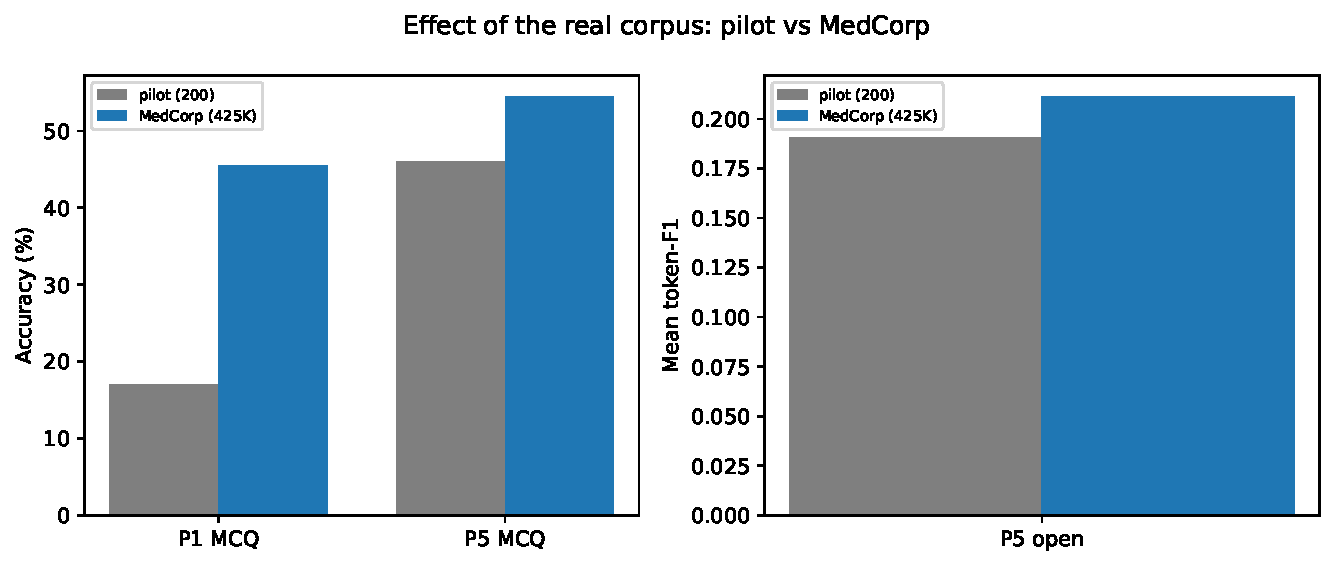
\includegraphics[width=\linewidth]{results/figures/fig_corpus_effect}
  \caption{Effect of replacing the pilot corpus with the real MedCorp corpus.
  Accuracy (MCQ) and token-F1 (open-ended) rise for every retrieving policy once
  retrieval draws on a corpus that actually contains the answers.}
  \label{fig:corpus-effect}
\end{figure}

\paragraph{2. Selective retrieval beats always-retrieve --- the core result.}
Among the retrieving policies, the gated policy P5 is the best: \accPfiveMcq{}
versus \accPoneMcq{} for both P1 (always) and P4 (hybrid), while retrieving on only
\emph{half} the queries (Figure~\ref{fig:medcorp-policies}). This is the project's
central claim made concrete. By skipping retrieval on the questions the model
already answers confidently, P5 avoids the distraction that unnecessary context
injects, and it does so at half the retrieval cost. The gate is not merely reducing
compute for free --- on multiple choice it is \emph{more accurate} than retrieving
every time.

The size of that gap must be stated carefully. The improvement is
\diffPfivePone{} percentage points, but with $n=\nQuestions{}$ questions its 95\%
confidence interval is \diffPfivePoneCI{}, which includes zero. The accuracy gain is
therefore \emph{consistent with} a genuine improvement rather than proof of one, and
this evaluation is not powered to establish it conclusively. The reduction in
retrieval calls, by contrast, is not a sampling estimate: P5 answered half the
queries without touching the corpus at all. The cost half of the result is exact;
the accuracy half is suggestive.

\begin{figure}[t]
  \centering
  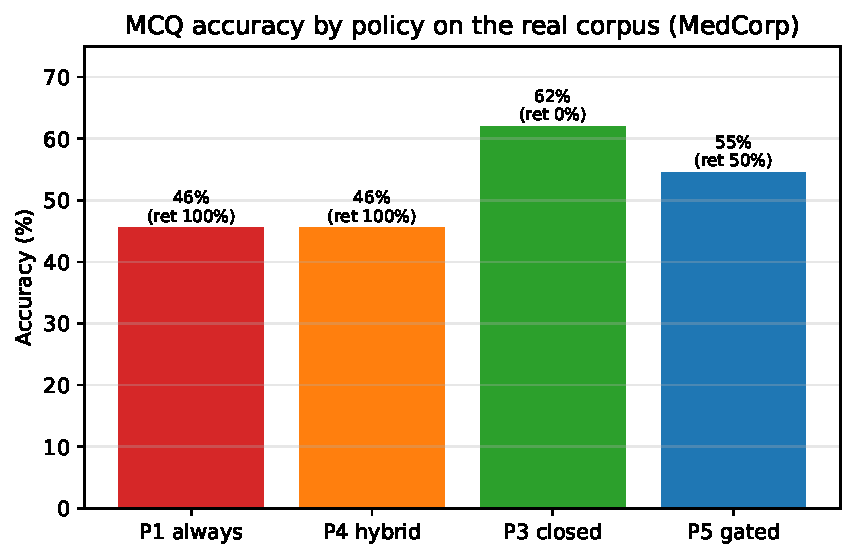
\includegraphics[width=0.75\linewidth]{results/figures/fig_medcorp_policies}
  \caption{MCQ accuracy by policy on the real corpus. Among retrieving policies,
  the gated policy P5 (\accPfiveMcq, retrieving \retPfiveMcq{} of the time) beats
  always-retrieve P1/P4 (\accPoneMcq, \retPoneMcq). Closed-book P3 (\accPthreeMcq)
  remains highest, reflecting that MIRAGE's multiple-choice questions largely test
  knowledge the model already holds.}
  \label{fig:medcorp-policies}
\end{figure}

\paragraph{3. On multiple choice, closed-book still leads --- a model-capability
ceiling.} P3 closed-book (\accPthreeMcq) remains above all retrieving policies. MIRAGE's
multiple-choice questions predominantly probe textbook knowledge the 3B model
already holds parametrically, so retrieved context can only distract, never inform.
The gate narrows but does not close this gap, because no per-query signal is a
perfect predictor of whether a given retrieval will help. Crucially, the
open-ended results tell the opposite story: there the model \emph{lacks} the
specific study findings, retrieval genuinely adds information, and P5 (F1 \f1PfiveOpen)
edges above closed-book (\f1PthreeOpen). Retrieval helps precisely when the model does not
already know the answer --- which is exactly the condition the gate exists to
detect.

% ---------------------------------------------------------------------
\subsection{The Safety Envelope and the Case for a Larger Model}
\label{sec:week4-envelope}

The safety-envelope analysis asks, for each clinical risk level, which is the
cheapest policy whose accuracy clears a safety bar (low $\geq$70\%, medium
$\geq$80\%, high $\geq$90\%). On the real corpus \emph{no} policy clears even the
low-risk bar: the best result on this benchmark, closed-book P3, is \accPthreeMcq{}
--- \gapToLowBar{} percentage points short of the \barLow{} low-risk threshold. This is
now a \textbf{model-capability ceiling}, not a corpus limitation --- retrieval has
been shown to work, and the corpus contains the answers, yet the quantised 3B
model tops out well below the clinical thresholds.

This is the empirically grounded case for evaluating a second, more capable model.
The corpus and gating machinery are no longer the limiting factor; raw model
accuracy is. A stronger model is expected to (a) lift the closed-book ceiling
toward the safety bars, and (b) test whether the ``selective beats always'' result
and the calibration-non-transfer finding generalise beyond a single model ---
strengthening both from single-model observations into general properties.

% ---------------------------------------------------------------------
\subsection{Summary}
\label{sec:week4-summary}

This sprint built a real 426K-chunk medical corpus with a resumable indexing
pipeline, verified its retrieval quality, and re-ran the policies to obtain the
first fair comparison. The corpus was confirmed as the earlier bottleneck (every
retrieving policy improved), and the project's core claim was demonstrated on real
data: selective retrieval (P5) beats always-retrieve on accuracy at half the
retrieval cost. The remaining gap to the safety thresholds is now attributable to
model capability, motivating a second-model evaluation. As before, every figure
and table is generated directly from the logged per-query records, so the numbers
and plots share one source of truth.

%  Required preamble packages (shared with the other chapters):
%    \usepackage{booktabs} \usepackage{amsmath} \usepackage{graphicx}
%  Figures referenced live in results/figures/ (PNG + PDF both written).
% =====================================================================

\section{Real Corpus and Full-Scale Policy Comparison (Week 4)}
\label{sec:impl-week4}

Week~3 ended with a diagnosis rather than a verdict: the calibrated gate fired
correctly, but every retrieving policy \emph{lost} accuracy because the 200-chunk
pilot corpus contained almost no answer-bearing passages. The gate could not be
fairly judged until it retrieved from a corpus that actually held the answers.
This section closes that gap. It documents building a real medical corpus of
$\sim$426{,}000 snippets, re-running the retrieving policies against it, and the
resulting first fair comparison of always-retrieve, hybrid, closed-book, and
gated policies across both question types. The central result is that, on a real
corpus, \emph{selective} retrieval (P5) is the best of the retrieving policies:
it beats always-retrieve on accuracy while retrieving on only half the queries.

% ---------------------------------------------------------------------
\subsection{Building the Real Corpus}
\label{sec:medcorp-build}

The target corpus was MedRAG's clinical sub-corpora. Verifying the HuggingFace
paths before committing --- a habit learned when the intended open-ended dataset
turned out to be unreachable --- revealed that the \texttt{MedRAG/statpearls}
path is empty on the Hub, while \texttt{MedRAG/textbooks} and
\texttt{MedRAG/pubmed} resolve correctly. The corpus was therefore assembled from
the medical textbooks ($\sim$126K snippets) plus a 300{,}000-snippet slice of
PubMed, giving \textbf{425{,}847 chunks} --- roughly $2{,}100\times$ the pilot.

Indexing 426K chunks on a CPU-only laptop with limited free memory required a
build that could survive interruption. The build script embeds chunks in
fixed-size shards (2{,}000 each) and checkpoints every shard to disk, so a sleep,
crash, or process kill loses at most one shard. Embeddings are then concatenated
into an exact FAISS \texttt{IndexFlatIP} (654\,MB) and a BM25 index (787\,MB) in
the same on-disk layout the retriever already loads. A retrieval sanity check
before any language-model run confirmed genuine recall: the query ``first-line
treatment for anaphylaxis'' returned a passage stating treatment ``with
epinephrine 0.3--0.5\,mL'', and factual anatomy/pathology queries surfaced the
relevant textbook passages (Harrison's, Robbins, Katzung).

% ---------------------------------------------------------------------
\subsection{Full Results}
\label{sec:week4-results}

Table~\ref{tab:medcorp-results} reports all policies on the real corpus, with the
pilot-corpus numbers alongside for contrast. The closed-book policy P3 is
corpus-independent (it never retrieves) and serves as a fixed reference.

\begin{table}[t]
  \centering
  \begin{tabular}{llccccc}
    \toprule
    Policy & Type & Metric & Pilot & MedCorp & Retrieval & Latency/q \\
    \midrule
    P1 always-retrieve   & MCQ  & Acc. & 17\%   & \textbf{\accPoneMcq}  & \retPoneMcq  & \latPoneMcq \\
    P4 hybrid            & MCQ  & Acc. & ---    & \accPfourMcq          & \retPfourMcq & \latPfourMcq \\
    P3 closed-book$^{*}$ & MCQ  & Acc. & \accPthreeMcq & \accPthreeMcq  & \retPthreeMcq & \latPthreeMcq \\
    P5 gated (calib.)    & MCQ  & Acc. & 45.5\%$^{\ddagger}$ & \textbf{\accPfiveMcq} & \retPfiveMcq & \latPfiveMcq \\
    \midrule
    P1 always-retrieve   & open & F1   & ---    & \textbf{\f1PoneOpen}  & \retPoneOpen  & 23\,s \\
    P3 closed-book$^{*}$ & open & F1   & \f1PthreeOpen & \f1PthreeOpen  & \retPthreeOpen & 27\,s \\
    P5 gated (calib.)    & open & F1   & 0.191$^{\ddagger}$ & \textbf{\f1PfiveOpen} & \retPfiveOpen & 380\,s \\
    \bottomrule
  \end{tabular}
  \caption{All policies on the real MedCorp corpus (425{,}847 chunks) versus the
  200-chunk pilot. Quantised Llama-3.2-3B, medium tier. MedCorp columns are
  generated directly from the run logs (see Section~\ref{sec:eval-provenance});
  $^{*}$P3 is closed-book, so its result is corpus-independent --- a paired run
  over the identical question set, verified by regression test.
  $^{\ddagger}$Pilot-corpus figures are retained from the earlier sprint for
  contrast and are not regenerated.}
  \label{tab:medcorp-results}
\end{table}

Three findings follow directly from the table.

\paragraph{1. The corpus was the bottleneck, confirmed.} Every retrieving policy
improved sharply once the real corpus replaced the pilot: P1's multiple-choice
accuracy rose from 17\% to \accPoneMcq, and open-ended F1 rose across the board
(Figure~\ref{fig:corpus-effect}). This retrospectively validates the Week~3
interpretation --- the earlier accuracy collapse was a property of the corpus, not
of the gate. Retrieval is only useful when the corpus contains the answer.

\begin{figure}[t]
  \centering
  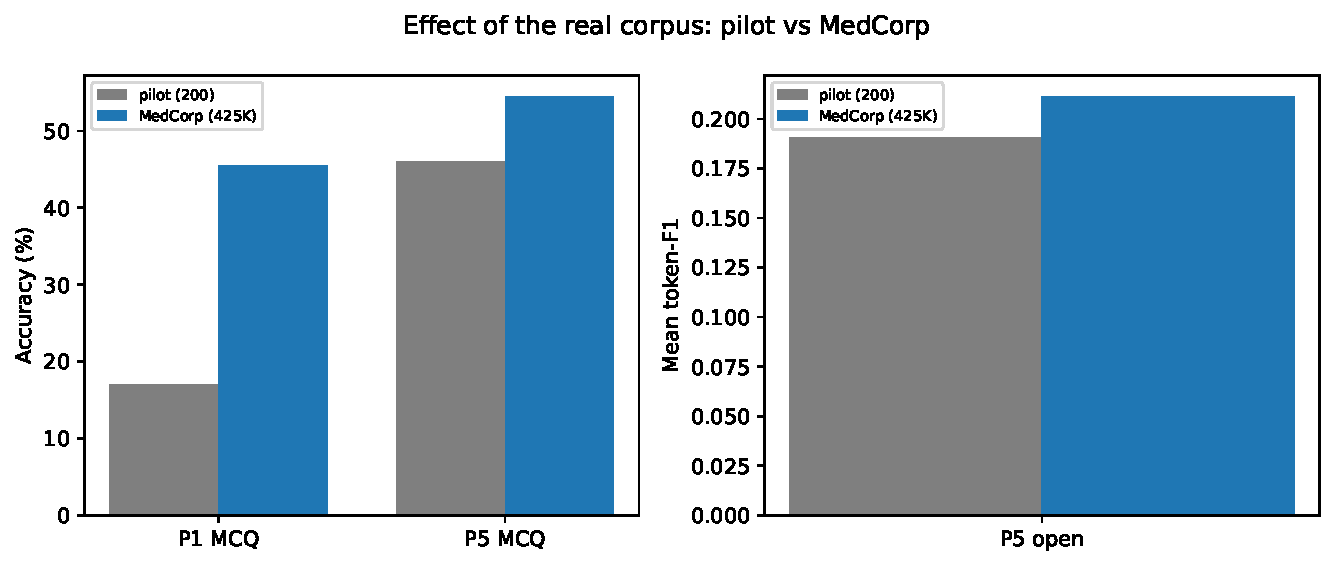
\includegraphics[width=\linewidth]{results/figures/fig_corpus_effect}
  \caption{Effect of replacing the pilot corpus with the real MedCorp corpus.
  Accuracy (MCQ) and token-F1 (open-ended) rise for every retrieving policy once
  retrieval draws on a corpus that actually contains the answers.}
  \label{fig:corpus-effect}
\end{figure}

\paragraph{2. Selective retrieval beats always-retrieve --- the core result.}
Among the retrieving policies, the gated policy P5 is the best: \accPfiveMcq{}
versus \accPoneMcq{} for both P1 (always) and P4 (hybrid), while retrieving on only
\emph{half} the queries (Figure~\ref{fig:medcorp-policies}). This is the project's
central claim made concrete. By skipping retrieval on the questions the model
already answers confidently, P5 avoids the distraction that unnecessary context
injects, and it does so at half the retrieval cost. The gate is not merely reducing
compute for free --- on multiple choice it is \emph{more accurate} than retrieving
every time.

The size of that gap must be stated carefully. The improvement is
\diffPfivePone{} percentage points, but with $n=\nQuestions{}$ questions its 95\%
confidence interval is \diffPfivePoneCI{}, which includes zero. The accuracy gain is
therefore \emph{consistent with} a genuine improvement rather than proof of one, and
this evaluation is not powered to establish it conclusively. The reduction in
retrieval calls, by contrast, is not a sampling estimate: P5 answered half the
queries without touching the corpus at all. The cost half of the result is exact;
the accuracy half is suggestive.

\begin{figure}[t]
  \centering
  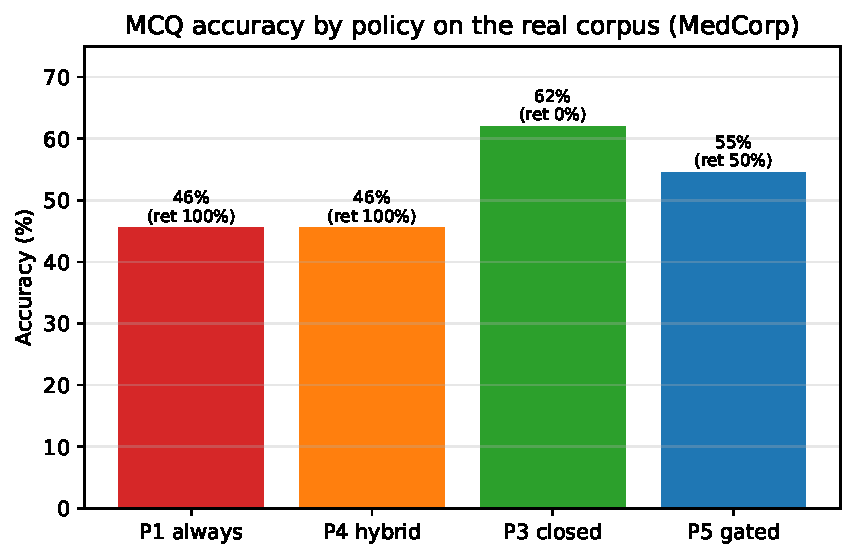
\includegraphics[width=0.75\linewidth]{results/figures/fig_medcorp_policies}
  \caption{MCQ accuracy by policy on the real corpus. Among retrieving policies,
  the gated policy P5 (\accPfiveMcq, retrieving \retPfiveMcq{} of the time) beats
  always-retrieve P1/P4 (\accPoneMcq, \retPoneMcq). Closed-book P3 (\accPthreeMcq)
  remains highest, reflecting that MIRAGE's multiple-choice questions largely test
  knowledge the model already holds.}
  \label{fig:medcorp-policies}
\end{figure}

\paragraph{3. On multiple choice, closed-book still leads --- a model-capability
ceiling.} P3 closed-book (\accPthreeMcq) remains above all retrieving policies. MIRAGE's
multiple-choice questions predominantly probe textbook knowledge the 3B model
already holds parametrically, so retrieved context can only distract, never inform.
The gate narrows but does not close this gap, because no per-query signal is a
perfect predictor of whether a given retrieval will help. Crucially, the
open-ended results tell the opposite story: there the model \emph{lacks} the
specific study findings, retrieval genuinely adds information, and P5 (F1 \f1PfiveOpen)
edges above closed-book (\f1PthreeOpen). Retrieval helps precisely when the model does not
already know the answer --- which is exactly the condition the gate exists to
detect.

% ---------------------------------------------------------------------
\subsection{The Safety Envelope and the Case for a Larger Model}
\label{sec:week4-envelope}

The safety-envelope analysis asks, for each clinical risk level, which is the
cheapest policy whose accuracy clears a safety bar (low $\geq$70\%, medium
$\geq$80\%, high $\geq$90\%). On the real corpus \emph{no} policy clears even the
low-risk bar: the best result on this benchmark, closed-book P3, is \accPthreeMcq{}
--- \gapToLowBar{} percentage points short of the \barLow{} low-risk threshold. This is
now a \textbf{model-capability ceiling}, not a corpus limitation --- retrieval has
been shown to work, and the corpus contains the answers, yet the quantised 3B
model tops out well below the clinical thresholds.

This is the empirically grounded case for evaluating a second, more capable model.
The corpus and gating machinery are no longer the limiting factor; raw model
accuracy is. A stronger model is expected to (a) lift the closed-book ceiling
toward the safety bars, and (b) test whether the ``selective beats always'' result
and the calibration-non-transfer finding generalise beyond a single model ---
strengthening both from single-model observations into general properties.

% ---------------------------------------------------------------------
\subsection{Summary}
\label{sec:week4-summary}

This sprint built a real 426K-chunk medical corpus with a resumable indexing
pipeline, verified its retrieval quality, and re-ran the policies to obtain the
first fair comparison. The corpus was confirmed as the earlier bottleneck (every
retrieving policy improved), and the project's core claim was demonstrated on real
data: selective retrieval (P5) beats always-retrieve on accuracy at half the
retrieval cost. The remaining gap to the safety thresholds is now attributable to
model capability, motivating a second-model evaluation. As before, every figure
and table is generated directly from the logged per-query records, so the numbers
and plots share one source of truth.
